\lab{HIV Treatment Using Optimal Control}{HIV Treatment Using Optimal Control}
\label{lab:hiv}


\section*{Introduction}
    Viruses are the cause of many common illnesses in society today, such as ebola, influenza, the common cold, and Human Immunodeficiency Virus (HIV). Viruses are not considered to be living organisms as they cannot reproduce on their own. Instead they inject their genes in the form of DNA or RNA into a host's genome. They then use the cell's ribosomes and proteins to make the protein coat and replicate their genes. At the end they lyse the cell (tear it apart) and release many virus particles to infect other cells.\par
    The body has an adaptive immune system which learns to recognize viruses and bacteria and their hosts, and how to destroy them. A major component of this system are T cells. These cells perform many necessary functions such as recognizing invaders, destroying infected cells, and remembering previous infections long after recovery. Of particular interest is the helper T cell, also known as the CD4+T cell, due to a protein found on its surface which regulates the immune responses. HIV is unique in that it specifically targets this particular type of T cell. This means that the system responsible for fighting infections is specifically targeted.\par
    This loss of CD4+T cells is what causes Acquired Immune Deficiency Syndrome (AIDS). Note that AIDS itself is not an infection, which is a common misconception among the population. Due to the lack of T cells to recognize viruses and bacteria, the body becomes susceptible to other forms of infection. Whereas most people are easily able to shake off a common cold, someone suffering from the advanced stages of AIDS will be at serious risk of dying. Since AIDS comes from a loss of T cells, it may be several years before the host notices the effects of the infection. This enables the HIV virus to spread more easily since the host might not realize they are infected and continue in whatever behavior made them susceptible to the infection initially.\par
   Currently there is no cure or vaccine for HIV. However, there are treatments that reduce the virus and bolster the immune system by increasing the CD4+T cell count. Since these treatments can be expensive and often have negative side effects, it is important to optimize the amount of drugs used. Sometimes combinations of these drugs are used to provide a better effect. In this lab we will use optimal control to find the optimal dosage of a two-drug combination\footnote{\textit{SHORT COURSES ON THE MATHEMATICS OF BIOLOGICAL COMPLEXITY}, Web. 15 Apr. 2015 http://www.math.utk.edu/~lenhart/smb2003.v2.html.} \footnote{`Immunotherapy of HIV-1 Infection', Kirschner, D. and Webb, G. F., Journal of Biological Systems, 6(1), 71-83 (1998)}.
   
   % \begin{thebibliography}{9}
% 
% \bibitem{paper}
% "SHORT COURSES ON THE MATHEMATICS OF BIOLOGICAL COMPLEXITY." \textit{SHORT COURSES ON THE MATHEMATICS OF BIOLOGICAL COMPLEXITY}, Web. 15 Apr. 2015 http://www.math.utk.edu/~lenhart/smb2003.v2.html.

% \bibitem{constants}
% .
% \end{thebibliography}
   
\begin{problem}
Explain what makes the HIV virus unique. What are the consequences of this? What is AIDS?
\label{problem:hiv:virusunderstanding}
\end{problem}

\begin{problem}
How is AIDS treated and what are the considerations for treatment?
\label{problem:hiv:treatment}
\end{problem}

\section*{Derivation of Control}
First we begin by writing the state system, the equations that describe the changes in T cells and viruses:
\begin{align*}
\frac{\it{d}T(t)}{\it{dt}} &= s_1 - \frac{s_2V(t)}{B_1+V(t)} - \mu T(t)-kV(t)T(t)+u_1(t)T(t), \\
\frac{\it{d}V(t)}{\it{dt}} &= \frac{gV(t)}{B_2+V(t)}(1-u_2(t)) - cV(t)T(t).
\end{align*}
To these equations we add initial conditions $T(0)=T_0$ and $V(0)=V_0$, where $T$ represents the concentration of $CD4^+T$ cells and $V$ the concentration of HIV particles. 
The term $s_1-\frac{s_2V(t)}{B_1+V(t)}$ is the source/proliferation of unaffected T cells,
$\mu T(t)$ the natural loss of T cells, $kV(t)T(t)$ the loss of T cells by infection. 
$\frac{gV(t)}{B_2+V(t)}$ represents the viral contribution to plasma, and $cV(t)T(t)$ the viral loss.

We now seek to maximize the functional 
\[
J(u_1,u_2) = \int_0^{t_f}[T-(A_1u_1^2+A_2u_2^2)]\it{dt}.
\]
This functional considers i) the benefit of T cells, and ii) the systematic costs of drug treatments.
The constants $A_1$ and $A_2$ represent scalars to adjust the size of terms coming from $u_1^2$ and $u_2^2$ respectively. 
We seek an optimal control $u_1^*,u_2^*$ satisfying
\[
J(u_1^*,u_2^*)=\max\{J(u_1,u_2)|(u_1,u_2)\in U\},
\]
where $U=\{(u_1,u_2)|u_i $ is measurable $,\,a_i\le u_i \le b_i$, $t\in[0,t_f]$ for $i=1,2\}$.
 
\section*{Optimality System}
The Hamiltonian is defined as:
\begin{align*}
	H = [T-(A_1u_1^2+A_2u_2^2)]&+\lambda_1\Big[ s_1 - \frac{s_2V}{B_1+V}-\mu T-kVT+u_1T \Big] \\
	&+ \lambda_2 \Big[\frac{g(1-u_2)V}{B_2+V}-cVT\Big].
\end{align*}
Note that the costate is represented with $\lambda$ instead of $p$. Now based on what we know from class we have:
\begin{align*}
\lambda_1^{'} &=-\frac{\partial H}{\partial T} =  -1+\lambda_1[\mu+kV^*-u_1^*]+\lambda_2cV^*,\\
\lambda_2^{'} &= -\frac{\partial H}{\partial V} = \lambda_1\Big[\frac{B_1s_2}{(B_1+V^*)^2}+kT^*\Big] -\lambda_2\Big[\frac{B_2g(1-u_2^*)}{B_2+V^*)^2}-cT^*\Big].
\end{align*}

The transversality conditions are $\lambda_1(t_f)=\lambda_2(t_f)=0$, with $T(0)=T_0$ and $V(0)=V_0$. 
%Also 
%$$u_1^* = min\Bigg\{max\Bigg\{a_1,\frac{1}{2A_1}(\lambda_1T^*(t))\Bigg\},b_1\Bigg\}$$
%$$u_2^* = min\Bigg\{max\Bigg\{a_2,\frac{-\lambda_2}{2A_2}\frac{V*(t)}{(B_2+V^*(t))}\Bigg\},b_2\Bigg\}$$
%The optimality equations are:
%$$\frac{\partial H}{\partial u_1} = -2A_1u_1^*(t)+\lambda_1T^*(t)=0$$
%$$\frac{\partial H}{\partial u_2} = -2A_2u_2^*(t)+\lambda_2\big[\frac{-gV^*(t)}{B_2+V^*(t)}\big
From these conditions we obtain
\begin{align*}
u_1^*(t) &= \frac{1}{2A_1}\left[\lambda_1T^*(t)\right],\\
u_2^*(t) &= \frac{1}{2A_2}\left[-\lambda_2\frac{gV^*(t)}{B_2+V^*(t)}\right].
\end{align*}
From the bounds on the controls we have
\begin{align*}
	\begin{split}
		u_1^*(t)&=\min\left\{\max\{a_1,\frac{1}{2A_1}(\lambda_1T^*(t))\},b_1\right\},\\
		u_2^*(t)&=\min\left\{\max\{a_2,-\frac{\lambda_2}{2A_2}\frac{gV^*(t)}{B_2+V^*(t)}\},b_2\right\}.
	\end{split}
\end{align*}
This gives us the optimal system
\begin{align*}
T'&=s_1-\frac{s_2V}{B_1+V}-\mu T-kVT+\min\{\max\{a_1,\frac{1}{2A_1}(\lambda_1T)\},b_1\}T,\\
V'&=\frac{g(1-\min\{\max\{a_2,\frac{-\lambda_2}{2A_2}\frac{gV}{B_2+V}\},b_2\})V}{B_2+V}-cVT,\\
\lambda_1'&=-1+\lambda_1\left[\mu+kV-\min\{\max\{a_1,\frac{1}{2A_1}(\lambda_1T)\},b_1\}\right]+\lambda_2cV,\\
\lambda_2'&=\lambda_1\left[\frac{B_1s_2}{(B_1+V)^2}+kT\right]-\lambda_2\left[\frac{B_2g(1-\min\{\max\{a_2,\frac{-\lambda_2}{2A_2}\frac{V}{B_2+V}\},b_2\})}{(B_2+V)^2}-cT\right],
\end{align*}
with end conditions $\lambda_1(t_f)=\lambda_2(t_f)=0$, and $T(0)=T_0,V(0)=V_0$.

\section*{Creating a Numerical Solver}

We iteratively solve for our control $u$. In each iteration we solve our state equations and our costate equations numerically, then use those to find our new control. Lastly, we check to see if  our control has converged. To solve each set of differential equations, we will use the RK4 solver from a previous lab with one minor adjustment. Our state equations depend on $u$, and our costate equations depend on our state equations. Therefore, we will pass another parameter into the function that RK4 takes in that will index the arrays our equations depend on.

\begin{lstlisting}
# Dependencies for this lab's code:
import numpy as np
from matplotlib import pyplot as plt

#Code from RK4 Lab with minor edits				
def initialize_all(y0, t0, t, n):
    """ An initialization routine for the different ODE solving
    methods in the lab. This initializes Y, T, and h. """
    if isinstance(y0, np.ndarray):
        Y = np.empty((n, y0.size)).squeeze()
    else:
        Y = np.empty(n)
    Y[0] = y0
    T = np.linspace(t0, t, n)
    h = float(t - t0) / (n - 1)
    return Y, T, h

def RK4(f, y0, t0, t, n):
    """ Use the RK4 method to compute an approximate solution
    to the ODE y' = f(t, y) at n equispaced parameter values from t0 to t
    with initial conditions y(t0) = y0.
    
    y0 is assumed to be either a constant or a one-dimensional numpy array.
    t and t0 are assumed to be constants.
    f is assumed to accept three arguments.
    The first is a constant giving the value of t.
    The second is a one-dimensional numpy array of the same size as y.
    The third is an index to the other arrays.
    
    This function returns an array Y of shape (n,) if
    y is a constant or an array of size 1.
    It returns an array of shape (n, y.size) otherwise.
    In either case, Y[i] is the approximate value of y at
    the i'th value of np.linspace(t0, t, n).
    """
    Y,T,h = initialize_all(y0,t0,t,n)
    for i in xrange(n-1):
        K1 = f(T[i],Y[i],i)
        K2 = f(T[i]+h/2.,Y[i]+h/2.*K1,i)
        K3 = f(T[i]+h/2.,Y[i]+h/2.*K2,i)
        K4 = f(T[i+1],Y[i]+h*K3,i)
        Y[i+1] = Y[i] + h/6.*(K1+2*K2 +2*K3+K4)
    return Y
\end{lstlisting}

\begin{problem}
Create a function that defines the state equations and returns both equations in a single array. The function should be able to be passed into the RK4 solver. This function can depend on the global variables defined below.

\begin{lstlisting}
# define constants
s_1 = 2.
s_2 = 1.5
mu = 0.002
k = 0.000025
g = 30.
c = 0.007
B_1 = 14
B_2 = 1

# initialize global variables, state, costate, and u.
state = np.zeros((n,2))
state0 = np.array([T0, V0])
	
costate = np.zeros((n,2))
costate0 = np.zeros(2)

u=np.zeros((n,2))
u[:,0] += .02
u[:,1] += .9

# define state equations
def state_equations(t,y,i):
	'''
	Parameters
	---------------
	t : float
		the time
	y : ndarray (2,)
		the T cell concentration and the Virus concentration at time t
	i : int
		index for the global variable u.
	Returns
	--------------
	y_dot : ndarray (2,)
		the derivative of the T cell concentration and the virus concentration at time t
	'''
	pass
\end{lstlisting}
\label{problem:hiv:state}
\end{problem}


The state equations work great in the RK4 solver; however, the costate equations have end conditions rather than initial conditions. Thus we want our RK4 solver to iterate backwards from the end to the beginning. An easy way to accomplish this is to define a function $ \hat{\lambda}_i(t)=\lambda_i(t_f - t).$ Then $\hat{\lambda}_i$ has the initial conditions $\hat{\lambda}_i(0) = \lambda_i(t_f)$. We get the new equations

\begin{align*}
\dot{\hat{\lambda}}_1(t) &=\lambda_1(t_f-t)\left(-\mu - kV(t_f-t) + u_{1}\right) - c\lambda_2(t_f-t)V(t_f-t) + 1, \\
\dot{\hat{\lambda}}_2(t) &= -\lambda_1(t_f-t)\left(\frac{s_2B_1}{(B_1+V(t_f-t))^2}+kT(t_f-t)\right) \\
&+ \lambda_2(t_f-t)\left(\frac{gB_2(1-u_2(t_f-t))}{(B_2 + V(t_f-t))^2} - cT(t_f-t)\right).
\end{align*}

These we can solve with our RK4 solver and recover the original costate equations by simply indexing the array backwards.

\begin{problem}
Create a function that defines the costate equations and returns both equations in a single array. The function should be able to be passed into the RK4 solver. Use the global variables as defined in Problem \ref{problem:hiv:state}.

\begin{lstlisting}
def lambda_hat(t,y,i):
	'''
	Parameters
	---------------
	t : float
		the time
	y : ndarray (2,)
		the lambda_hat values at time t
	i : int
		index for global variables, u and state.
	Returns
	--------------
	y_dot : ndarray (2,)
		the derivative of the lambda_hats at time t.
	'''
	pass
\end{lstlisting}

\label{problem:hiv:costateequations}
\end{problem}


\begin{figure}
\centering
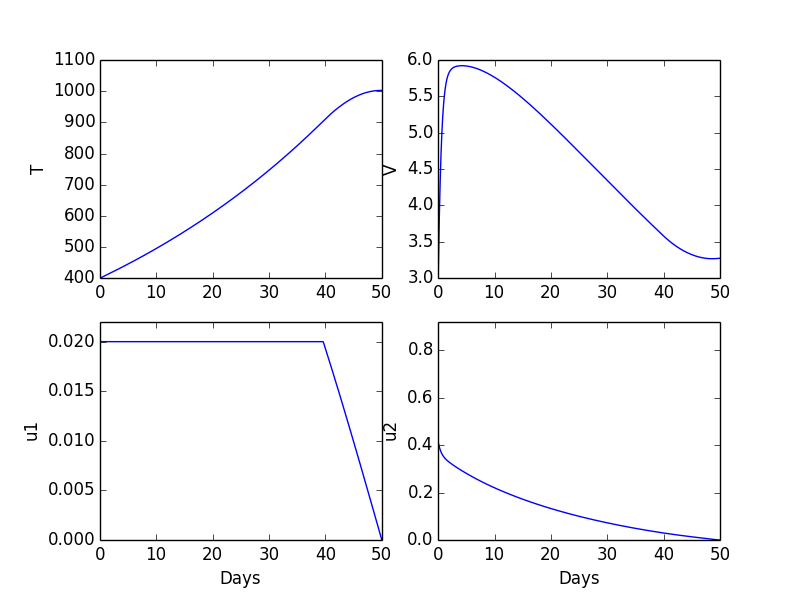
\includegraphics[width=5in]{solutions.png}
\caption{The solution to Problem \ref{problem:hiv:numericalsolver}.}
\label{fig:hiv:solutions}
\end{figure}



Finally, we can put these together to create our solver.
\begin{problem}
Create a numerical solver for the HIV two drug model using the code below.

\begin{lstlisting}
epsilon = 0.001
test = epsilon + 1

while(test > epsilon):
	oldu = u.copy();
    
	#solve the state equations with forward iteration
	#state = RK4(...)
    
	#solve the costate equations with backwards iteration
	#costate = RK4(...)[::-1]
	
	#solve for u1 and u2
    
	#update control
	u[:,0] = 0.5*(u1 + oldu[:,0])
	u[:,1] = 0.5*(u2 + oldu[:,1])

	#test for convergence
	test = abs(oldu - u).sum()
\end{lstlisting}

Run with the following parameter values:
\begin{lstlisting}
a_1, a_2 = 0, 0
b_1, b_2 = 0.02, 0.9
s_1, s_2 = 2., 1.5
\mu = 0.002
k = 0.000025
g = 30.
c = 0.007
B_1, B_2 = 14, 1
A_1, A_2 = 250000, 75
T_0, V_0 = 400, 3
t_f = 50
n = 1000
\end{lstlisting}
These constants come from both references cited at the end of this lab. Your solutions should match Figure \ref{fig:hiv:solutions}.
\label{problem:hiv:solver}

\label{problem:hiv:numericalsolver}
\end{problem}

In modern medicine, patients generally take combinations of five or more medications with different functions. These include Nucleotide Reverse Transcriptase Inhibitors, which prevent HIV inserting its genes into host DNA, Non-Nucleoside Reverse Transcriptase Inhibitors, which do the same job as NRTIs in a different fashion, Protease Inhibitors, which cut up replicated HIV strands, Fusion Inhibitors, which block the virus from entering the cells to begin with, and Integrase Inhibitors, which prevents the virus' replicated DNA from being inserted into a cell's DNA. These drugs often can interact with each other and have different side effects on the body. Also, doctors rotate medications as the body and virus develop immunity. 

% \begin{thebibliography}{9}
%
% \bibitem{paper}
% "SHORT COURSES ON THE MATHEMATICS OF BIOLOGICAL COMPLEXITY." \textit{SHORT COURSES ON THE MATHEMATICS OF BIOLOGICAL COMPLEXITY}. Web. 15 Apr. 2015. http://www.math.utk.edu/~lenhart/smb2003.v2.html.
%
% \bibitem{constants}
% Kirschner, D. and Webb, G. F., `Immunotherapy of HIV-1 Infection', Journal of Biological Systems, 6(1), 71-83 (1998).
% \end{thebibliography}

